\documentclass[12pt,a4j]{jarticle}

\makeatletter
  \def\@maketitle{%
  \newpage\null
  \vskip 2em%
  \begin{center}%
  \let\footnote\thanks
    {\LARGE \@title \par}%
    \vskip 1.5em%
  \end{center}% 追加
    \mbox{}\hfill%% 追加
    {\large
      \lineskip .5em%
      \begin{tabular}[t]{c}%
        \@author
      \end{tabular}\par}%
    \vskip 1em%
  \begin{flushright}% 追加
    {\large \@date}%
  \end{flushright}%
  \par\vskip 1.5em}
\makeatother

\usepackage[dvipdfmx]{graphicx}% 画像の読み込み
\usepackage{type1cm}% おまじない
\usepackage{url}% URL の記述のため
\usepackage[margin=3cm]{geometry}
\usepackage{setspace} % setspaceパッケージ 行間の設定
\usepackage{fancybox,ascmac}
\usepackage{comment} %コメントアウト用のパッケージ
\usepackage{tipa} %発音記号用

\setstretch{1.2} % ページ全体の行間を設定

\makeatletter
\def\mojiparline#1{
    \newcounter{mpl}
    \setcounter{mpl}{#1}
    \@tempdima=\linewidth
    \advance\@tempdima by-\value{mpl}zw
    \addtocounter{mpl}{-1}
    \divide\@tempdima by \value{mpl}
    \advance\kanjiskip by\@tempdima
    \advance\parindent by\@tempdima
}
\makeatother
\def\linesparpage#1{
    \baselineskip=\textheight
    \divide\baselineskip by #1
}


\setcounter{page}{0} %ページのスタート番号設定

% 一行あたり文字数の指定
\mojiparline{40}
% 1ページあたり行数の指定
\linesparpage{34}

\begin{document}

\begin{center}
{\huge 修士論文}
\vspace*{4.5cm}

{\LARGE\bf マルチエージェントシミュレーションによる \\}
{\LARGE\bf 不規則動詞の規則化に関する人口流入の影響} % ← 自分の研究テーマに置き換える
\vspace*{3cm}

\thispagestyle{empty} %ページ番号を表示させない
\end{center}

\newpage
%目次

\tableofcontents
\thispagestyle{empty} %ページ番号を表示させない
\newpage

\section{はじめに}\label{sec:intro}
\subsection{研究の目的}
現在の日常的に用いられている不規則動詞はおおよそ180語存在し、
会話の中に出現する動詞の約70\%が
不規則動詞である\cite{pinker}.これらの不規則動詞はOld English時代[AD 800 頃]に強変化動詞(strong verb)と呼ばれ主に母音が変化して活用していた.
Modern Englishでは例外も含め9クラスに分類され、クラス内にも細かい分類がある\cite{pinker2}.
しかし、不規則動詞には接尾辞[-ed]をつける規則的な活用に変化しているという現象が起こっている.
英語の歴史的な流れの中では、Old Englishから中期英語時代における海賊によるイングランドの侵略、ノルマン征服などの
人口流入を伴った言語接触により不規則動詞の規則化の誘発、またその加速が起こっている.\\
 本研究ではこの不規則動詞の規則化に対する人口流入の規模、頻度をシミュレーションによって検証することを目的とする.検証のために遺伝的アルゴリズム\cite{iba_ga}(以下GA)をベースに、エージェントコミュニケーションと変化
を進行させるような(外圧)を組み込んだモデルを作成し、複数世代を通したシミュレーションを行う.

\subsection{本論文の構成}

\newpage
\section{背景}\label{sec:back}

本章では英語の不規則動詞の言語的背景、また言語接触に関する歴史的背景について述べる.
言語学的背景では、英語の起源と時代区分について述べる.またOld English時代
に用いられていた強変化動詞について説明を行う.
不規則動詞の規則化に関する歴史的背景では、Viking(海賊)やノルマン征服などイングランドにおける侵略と
英語に与えた影響について述べる.


\subsection{言語学的背景}\label{sec:div}
本節では英語の不規則動詞について英語の起源と時代区分を含めて説明を行う.
また、

\subsubsection{英語の起源と時代区分}

はじめに英語の起源について述べる.
英語はProto-Indo-Europeanを起源とするゲルマン語派言語である\cite{eng_history}.
Proto-Indo-Europeanを起源とするその他の言語には、ケルト語派、イタリック語派などが
ある.Proto-Indo-Europeanの系統図を図\ref{fig:tree}に示す.

\begin{figure}[htbp]
 \centering
 \includegraphics[width=15cm]{lang_tree.eps}
 \caption{印欧語(Proto-Indo-European)族の系統図\cite{eng_history}より引用\label{fig:tree}}
\end{figure}

Proto-Indo-European語族には英語を含む
多くのヨーロッパ諸国の言語が含まれていることがわかる.
Proto-Indo-Europeanは現在は失われているが、紀元前4000年ごろに南ロシアに栄えていた
クルガン文化の担い手によって話されていたという説がある\cite{eng_history}.
その後、各地で方言化し諸言語へと進化していった.\\

次に古英語以降の時代区分について述べる.
英語の年代区分は、ノルマン征服など歴史的な事実を区切りに用いるが、
3区切りや6から7つに区切るモデルも存在する.
表\ref{tab:eng_div_table}に4つの時代に区切るモデル\cite{english_div}を示す.


\begin{table}[htbp]
 \centering
 \caption{英語の時代区分\label{tab:eng_div_table}}
 \small
 \begin{tabular}{l|c}
  \hline
  A.D 500 -1150 & Old English \\
  \hline
  A.D 1150 -1450 & Middle English \\
  \hline
  A.D 1450 -1700 & Early Modern English \\
  \hline
  A.D 1700 - & Modern English \\
  \hline
\end{tabular}
\end{table}

各時代について簡単に説明する.
Old English時代は大ブリテン島南部でアングル、サクソン、ジュート族によって言語が確立された時期である.
その後、ノルマン征服によってノルマンフランス語との接触による影響が出始めた時代
がMidle English時代である.活版印刷技術が西ヨーロッパに広がりはじめた時期がEarly Modern English時代、
アン女王の時代以降がModern English時代となる.\\
 第\ref{sec:div}節の区分においてOld English時代に母音交替によって活用していた動詞が不規則動詞
である.

\subsubsection{不規則動詞とは}\label{sec:strong_verb}
本節では現在の不規則動詞について、そのルーツと人間の過去形生成の
仕組みについて述べる.

\begin{itemize}
\item 強変化動詞
\end{itemize}

Old English時代に用いられていた動詞は母音交替によって活用していた強変化動詞、(-t/de)など歯茎音の接辞
によって活用する弱変化動詞、過去時制が現在形の意味も表す過去現在動詞やその他少数の不規則動詞
がある\cite{strong_verb}.現在不規則動詞と呼ばれるものは強変化動詞がルーツとされる.
強変化動詞の基本構造は[子音+母音+子音]であり、これに
\textipa{r\=\i d-an(不定詞), r\=ad(過去1形), rid-on(過去2形), rid-ed(過去分詞)}のように活用語尾がつく.
ここで、過去1形は過去単数1,3人称、過去2形は過去単数2人称および過去複数形である.
これら4つの形を作る中で母音交替が起こる.
強変化動詞にはその母音交替のパターンによってクラス分けが存在する.強変化動詞にも基本形と
基本形から派生した変異形が存在するが個々では基本形のみ扱うものとする.
表\ref{tab:strong_class}に例を示す.
\begin{table}[htb]
  \begin{center}
    \caption{母音交替パターンによるクラス分け\cite{strong_verb}を元に作成}
    \begin{tabular}{|c|c|c|} \hline
      類 & 不定形 & 母音交代系列 \\ \hline
      I & \textipa{r\=\i dan(to ride)} & \textipa{\=\i,\=a,i,i}  \\ \hline
      I\hspace{-.1em}I & \textipa{b\=eodan(to bid)} & \textipa{\=eo,\=ea,u,o} \\ \hline
      I\hspace{-.1em}I\hspace{-.1em}I.N & \textipa{bindan(to bind)} & \textipa{i,a,u,u}  \\\hline
      I\hspace{-.1em}I\hspace{-.1em}I.L1 & \textipa{helpan(to help)} & \textipa{e,ea,u,o}\\ \hline
      I\hspace{-.1em}I\hspace{-.1em}I.L2 & \textipa{weorpan(to throw)} & \textipa{eo,ea,u,o}\\ \hline
      I\hspace{-.1em}V & \textipa{beran(to bear)} & \textipa{e,\ae,\=\ae,e} \\ \hline
      V-1 & \textipa{metan(to measure)} & \textipa{e,\ae,\=\ae,e} \\ \hline
      V-2 & \textipa{giefan(to give)} & \textipa{ie,ea,\=ea,ie} \\ \hline
      V\hspace{-.1em}I & \textipa{faran(to go)} & \textipa{a,\=o,a} \\ \hline
      V\hspace{-.1em}I\hspace{-.1em}Ia & \textipa{h\=atan(to call)} & \textipa{\=a,\=e,\=a, etc...} \\ \hline
      V\hspace{-.1em}I\hspace{-.1em}Ib & \textipa{bannan(to summon)} & \textipa{a,\=eo,a}, etc.. \\ \hline 
      
    \end{tabular}
    \label{tab:strong_class}
  \end{center}
\end{table}

I, I\hspace{-.1em}I、I\hspace{-.1em}I\hspace{-.1em}I類は
それぞれ長母音、二重母音、母音+亮音(\textipa{鼻音n,m}, \textipa{流音l, r})の動詞である.
語幹母音が短母音でその末尾の音が流音\textipa{l,r}、鼻音\textipa{n,m}
である動詞がI\hspace{-.1em}V類、そうでない動詞がV類である. V\hspace{-.1em}I
はI\hspace{-.1em}V類とV類が混合したものである.
V\hspace{-.1em}I\hspace{-.1em}I類はかつてゴード語において畳音(zigzagなどの音を重ねるもの)を用いて過去形を
作る動詞であったものである.



\begin{itemize}
\item 過去形生成の仕組み
\end{itemize}
Jackendoff\cite{jack}によれば形態論的には規則動詞の過去形生成は生産的ルールであり、不規則動詞の過去形生成
は半生産的ルールである.ここで生産的という意味は、動詞に対してまったく規則的に行われるという事である.
英語の現在分詞(-ing)の生成は英語の動詞全てに例外なく行われる.つまり、生産的なルールは発話するときになって
その場で適用すればよく、長期記憶に蓄える必要はない.しかし、半生産的なルールはある程度長期記憶に蓄える
必要がある.不規則動詞の場合、母音交替にある程度のパターンは見られるものの完全に予想することはできない.
そのため、不規則動詞の過去形を使う場合は長期記憶にとどめておく必要がある.

またPinkerらはWord and Rule Theory\cite{pinker3}提唱した.概要図を図\ref{fig:word_rule}に示す.

\begin{figure}[htbp]
 \centering
 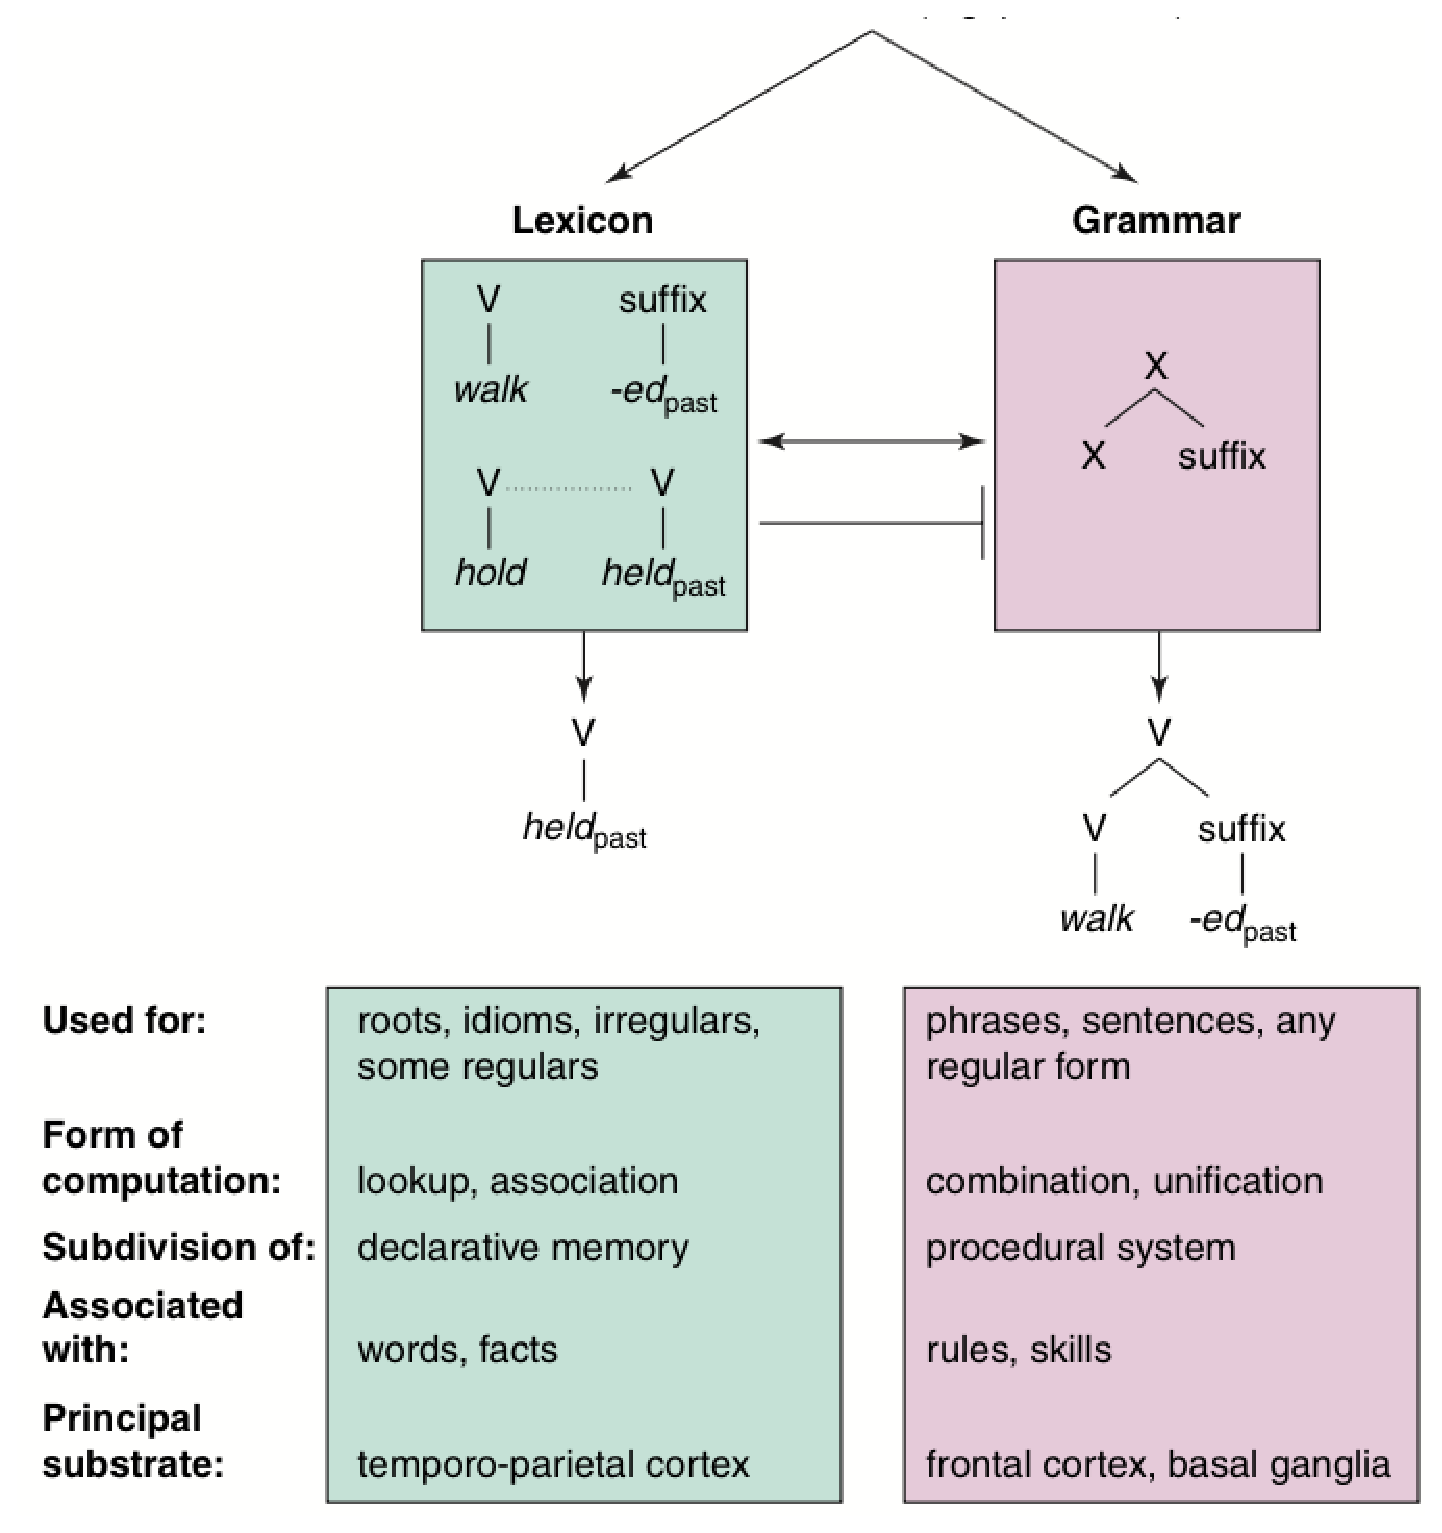
\includegraphics[width=8cm]{word-rule.eps}
 \caption{Word and Rule Theory\cite{pinker3}より引用\label{fig:word_rule}}
\end{figure}

図\ref{fig:word_rule}中のLexiconとは記憶の一部で形態素などを保持している.Grammarは形態素や単純な
語を組み合わせる能力である.またLexiconとGrammarには同時にアクセスできる.
例えばholdという語幹が入力された時(発話しようとした時)、Lexiconの中にholdの過去形と
マッチするheldが存在する場合、Grammar側で接尾辞edをつけて発話するという作業はストップさせられる.
よって発話はheldとなる. もし、なんらかの理由でheldを見つけられない場合Grammar側からの
発話となりedがついた過去形が生成される.heldを見つけられない理由としては、heldの頻度が
とても低いか0であること、子供のときに異なる形で記憶された、記憶にダメージをおったなど
が挙げられている.
不規則であった動詞が規則化される(edをつけて過去形を生成する)原因としても上記が
関係しているのではないかと指摘している.



\subsection{歴史的背景}\label{sec:history_back}
本節では実際の英語史において起こった人工流入や言語接触の影響\cite{english_div, philip, ziten}について述べる.

Old Englishは大ブリテン島でケルト人が使用していたとされているが、以下の侵略など
の歴史を通して形作られてきた言語である.
A.D400-550頃にゲルマン人の英国侵略
が始まり、アングル人(Angles)、サクソン人(Saxons)、ジュート人(Jutes)の部族も侵略に加わった\cite{ziten}.
この影響からOld English初期の語彙にはゲルマン系の語彙が多い.
また、A.D500-700にかけて英国にキリスト教が伝わった影響でラテン語の借用、または
そのままOld Englishに持ち込むといった現象が起こった.apostol(apostle)、cyrce(church)
などの教会用語が主である.\\
 A.D800-1066ごろにOld Englishに影響を与えたのは海賊(Viking)である.海賊はスウェーデン、ノルウェー、
デンマークに居住していたデーン人である.また海賊は古北欧語(ノルド語)話者であった.
海賊は主に商売や時には略奪行為を目的とし、英国の
東海岸を襲った.また、襲撃を繰り返すだけでなく英国に定住する者もいた.図\ref{fig:viking_nrman}
におおよその地域(青)を示す.
英国のアルフレッド大王は海賊と戦うこともあったが、やがて共存の道を開いていった.
その過程の中でノルド語はOld Englishに吸収されていくが、かなりの数の語をOld Englishの
中に残した.この時取り込まれた語はfellow, sky, to take, などの一般語、they-their-them
などの代名詞は今日でも使用されている.
この接触によってOld Englishでは三人称単数の語尾に[-s]をつけるようになった.
またこの時期に強変化動詞の規則化が始まったとされている.\\

 次にA.D1066-1345ごろのノルマン征服の影響について述べる.
Old Englishの後期に英国の王位継承をめぐって英国王室と北フランスのノルマンディ公国
の間で争いが起こった.争いはノルマンディ側の勝利で終了した(ノルマン征服).
図\ref{fig:viking_nrman}にノルマン人によって征服された地域(赤)のおおよその位置を示す.
そのため征服以降では、行政や軍事、司法などはフランス語で行われた.
Old Englishに及ぼした影響であるが、一部の同義語の交代や新語の流入が起こっている.
表\ref{tab:change}に同義語の交代の例を示す.

\begin{table}[htb]
  \begin{center}
    \caption{同義語の交代例\cite{ziten}より引用}
    \begin{tabular}{ccc} 
      以前の表現 & 以降の表現 &  \\ \hline
      preost & chapellain & 僧侶  \\ 
      fir\textipa{\dh}/gri\textipa{\dh} & pais & 平和\\
      unfi\textipa{\dh} & werre & 戦争 \\
      lufu & cherite & 愛
      
    \end{tabular}
    \label{tab:change}
  \end{center}
\end{table}

表\ref{tab:change}の語は完全に入れ替わったわけではなく、preost(priest), lufu(love)
としてModern Englishに残っている単語も存在する.
新語の流入ではbaron, champion, army, pawnなど爵位、軍事、司法用語などが
約1万語ほど流入したと考えられている.また、文法などの言語構造の簡略化や、海賊の影響
で始まった規則化傾向も上昇した.ノルマン征服後3世紀ほどでOld ~ Middle Englishは
復活し、英国の話し言葉となった.しかし、フランス語は書き言葉として吸収が続けられた.

 以上より、侵略、征服など様々な言語接触を経験していることが英語の特徴であると言える.


\begin{figure}[htbp]
 \centering
 \includegraphics[width=6cm]{viking_nrman.eps}
 \caption{海賊とノルマン人の居住、征服地域\label{fig:viking_nrman}}
\end{figure}

\newpage
\section{先行研究}\label{sec:pre}
本章では不規則動詞に関するコーパスを用いた統計的な研究について述べる.
不規則動詞の出現頻度と規則化の速度に関する研究では、
接尾辞edをつけることによって過去形を生成するようになる規則化が
コーパス内での出現頻度と時間の関数として導出した研究について述べる.\\
 語形変化に影響を及ぼす力に関する研究では、単語が古い形から
新しい形に変化するときに、変化を推し進めるような2つの力(内圧、外圧)
を数値的に求めた研究について述べる.


\subsection{不規則動詞の出現頻度と規則化の速度に関する研究}
\subsection{語形変化に影響を及ぼす力に関する研究}

\section{過去形獲得モデルの提案}\label{sec:model}
本章ではマルチエージェント環境の中で各エージェントが
コミュニケーションを通して共通の過去形を獲得するモデル
を提案する.このモデルを使用することで、規則化の速度や
その速度を引き起こす原因について考察できると考えられる.


\subsection{実験に必要な知識}
本節では提案モデルに必要となる知識について述べる.
マルチエージェントとは何か、またコミュニケーションの
目的と言語変化への関わりについて述べる.
マルチエージェント環境を現実世界の人間のつながりに近づけるために
使用する複雑ネットワークについも説明を行う.
また、人工的な動詞の過去形をどうやって生成しているのかアンケート調査
を行った研究とそれに付随して単語の音韻的距離を計測するアルゴリズムに
ついて述べる.
最後にエージェントの学習機構に用いる遺伝的アルゴリズムについて述べる.

\subsubsection{マルチエージェントとコミュニケーション}
\subsubsection{複雑ネットワークを用いた言語変化シミュレーション}
\subsubsection{人工的な不規則動詞に対する既存の母音活用の適用}
\subsubsection{MetaPhoneアルゴリズム}
\subsubsection{遺伝的アルゴリズム}


\section{実験}\label{sec:exp}
\section{実験結果と考察}\label{sec:kousatu}
\section{結論}\label{sec:concl}

\begin{thebibliography}{9}
\addcontentsline{toc}{section}{\refname}% 目次に追加
 \bibitem{pinker}
   \emph{Pinker, S. The irregular verbs. Landfall 83–85 (Autumn issue, 2000)}
 \bibitem{pinker2}
   \emph{Pinker, S , Prince, A. On language and connectionism: analysis of a parallel distributed processing model of language acquisition. Cognition 28,p73-193 (1988)}
 \bibitem{english_div}
   \emph{Tom McArthur, THE ENGLISH LANGUAGES, Cambridge University Press (1998), 英語系諸言語, 牧野武彦 監修, 山田 茂, 中本 恭平 訳, 三省堂 (2009)}
  \bibitem{eng_history}
    \emph{堀田隆一, 英語史で解きほぐす英語の誤解: 納得して英語を学ぶために. 中央大学出版部, (2011)}
 \bibitem{philip}
   \emph{Philip Gooden, THE STORY OF ENGLISH (2009), 物語 英語の歴史, 田口孝夫 監修, 悠書館 (2012)}
\bibitem{strong_verb}
  \emph{岩本忠. "古期英語強変化動詞の類別定義と韻構造: 基本型と変異型." (2006)}
 \bibitem{ziten}
   \emph{亀井孝, 河野六郎, 千野栄一. 言語学大辞典. Vol. 1. 三省堂, (1996)}
\bibitem{jack}
  \emph{Jackendoff, Ray. Foundations of language: Brain, meaning, grammar, evolution. Oxford University Press, (2002)}
\bibitem{pinker3}
\emph{Pinker, Steven, and Michael T. Ullman. "The past-tense debate." cognitive processing 5 (2002)}
 \bibitem{iba_ga}
   \emph{伊庭 斉志, 遺伝的アルゴリズムの基礎-GAの謎を解く オーム社(1994)}
  \bibitem{Lieberman}
    \emph{Erez Lieberman, Jean-Baptiste Michel, Joe Jackson, Tina Tang , Martin A. Nowak, Quantifying the evolutionary dynamics of language. Nature Vol449 (11 October 2007)}
  \bibitem{celex}
    \emph{CELEX http://wwwlands2.let.kun.nl/members/software/celex.html}
  \bibitem{scurve}
    \emph{Ghanbarnejad, Fakhteh, et al. Extracting information from S-curves of language change. Cornell University Library arXiv preprint arXiv:1406.4498 (2014)}
  \bibitem{spelling}
    \emph{Chris Upward, Spelling Reform in German. Journal of the Simplified Spelling Society, J21, 1997-1 pp22-24,36}
  \bibitem{google}
    \emph{Google Ngram Viewer, https://books.google.com/ngrams}
\end{thebibliography}

\end{document}
